\chapter{Planteamiento del problema} 

Hoy en día en México, la sociedad no tiene ningún interés por conocer o realizar actividades culturales. Tomaremos como actividades culturales a aquellas de aspecto artístico o histórico como obras de arte, literatura, música, danza, exposiciones y proyecciones audiovisuales. A continuación hablarémos sobre el contexto que rodea esta problemática, sus causas, consecuencias y la solución que proponemos.
\\[1pt]

\section{Contexto}
La diversidad cultural según el Movimiento Nacional por la Diversidad Cultural de México(MNDCM) es la múltiple cantidad de formas de expresión entre grupos y sociedades\cite{pp05}. La diversidad se manifiesta a través de distintos modos de creación artística, producción, difusión y distribución de dichas expresiones. La diversidad cultural es vital para el desarrollo de cualquier comunidad, pues es fuente de creatividad, innovación, originalidad, intercambio y enriquecimiento.
\\[1pt]

México es conocido por ser un país muy diverso culturalmente hablando. Cada estado posee su propia cultura regional, como la música, vestimenta tradicional, comida, entre otras cosas. Entre todos los estados del país podemos ver que existen grandes diferencias y aún así se comparte una misma identidad como país.
\\[1pt]

\section{Causas}

La ignorancia cultural del país se debe a que existe un desconocimiento de desarrollo social. Es decir que la sociedad del país tampoco tiene idea sobre su situación económica, capital humano, condiciones de salud, estado de la educación y condiciones de vida, todo esto llamado comúnmente como el bienestar social.
\\[1pt]

Existe una relación directa entre el desarrollo cultural y social. Pues ambas son debido al entorno y evolución de la sociedad que involucra. Con lo anterior deducimos que el desarrollo social favorece el desarrollo cultural.
\\[1pt]

En la última encuesta de Ipsos sobre Percepción\cite{pp04} se revela que tan errónea es la interpretación que las personas tienen sobre su desarrollo social. A partir de los datos recogidos en la encuesta y su comparación con datos reales, en temas acerca de los problemas y rasgos clave de la población de su país se elaboró la gráfica \ref{fig:ipso}. Se puede observar que México ocupa el duodécimo lugar (empatado con Corea del sur) en ignorancia total de su desarrollo como país. Entonces sí existe una ignorancia sobre desarrollo social en México.
\\[1pt]

\begin{figure}
	\centering 
	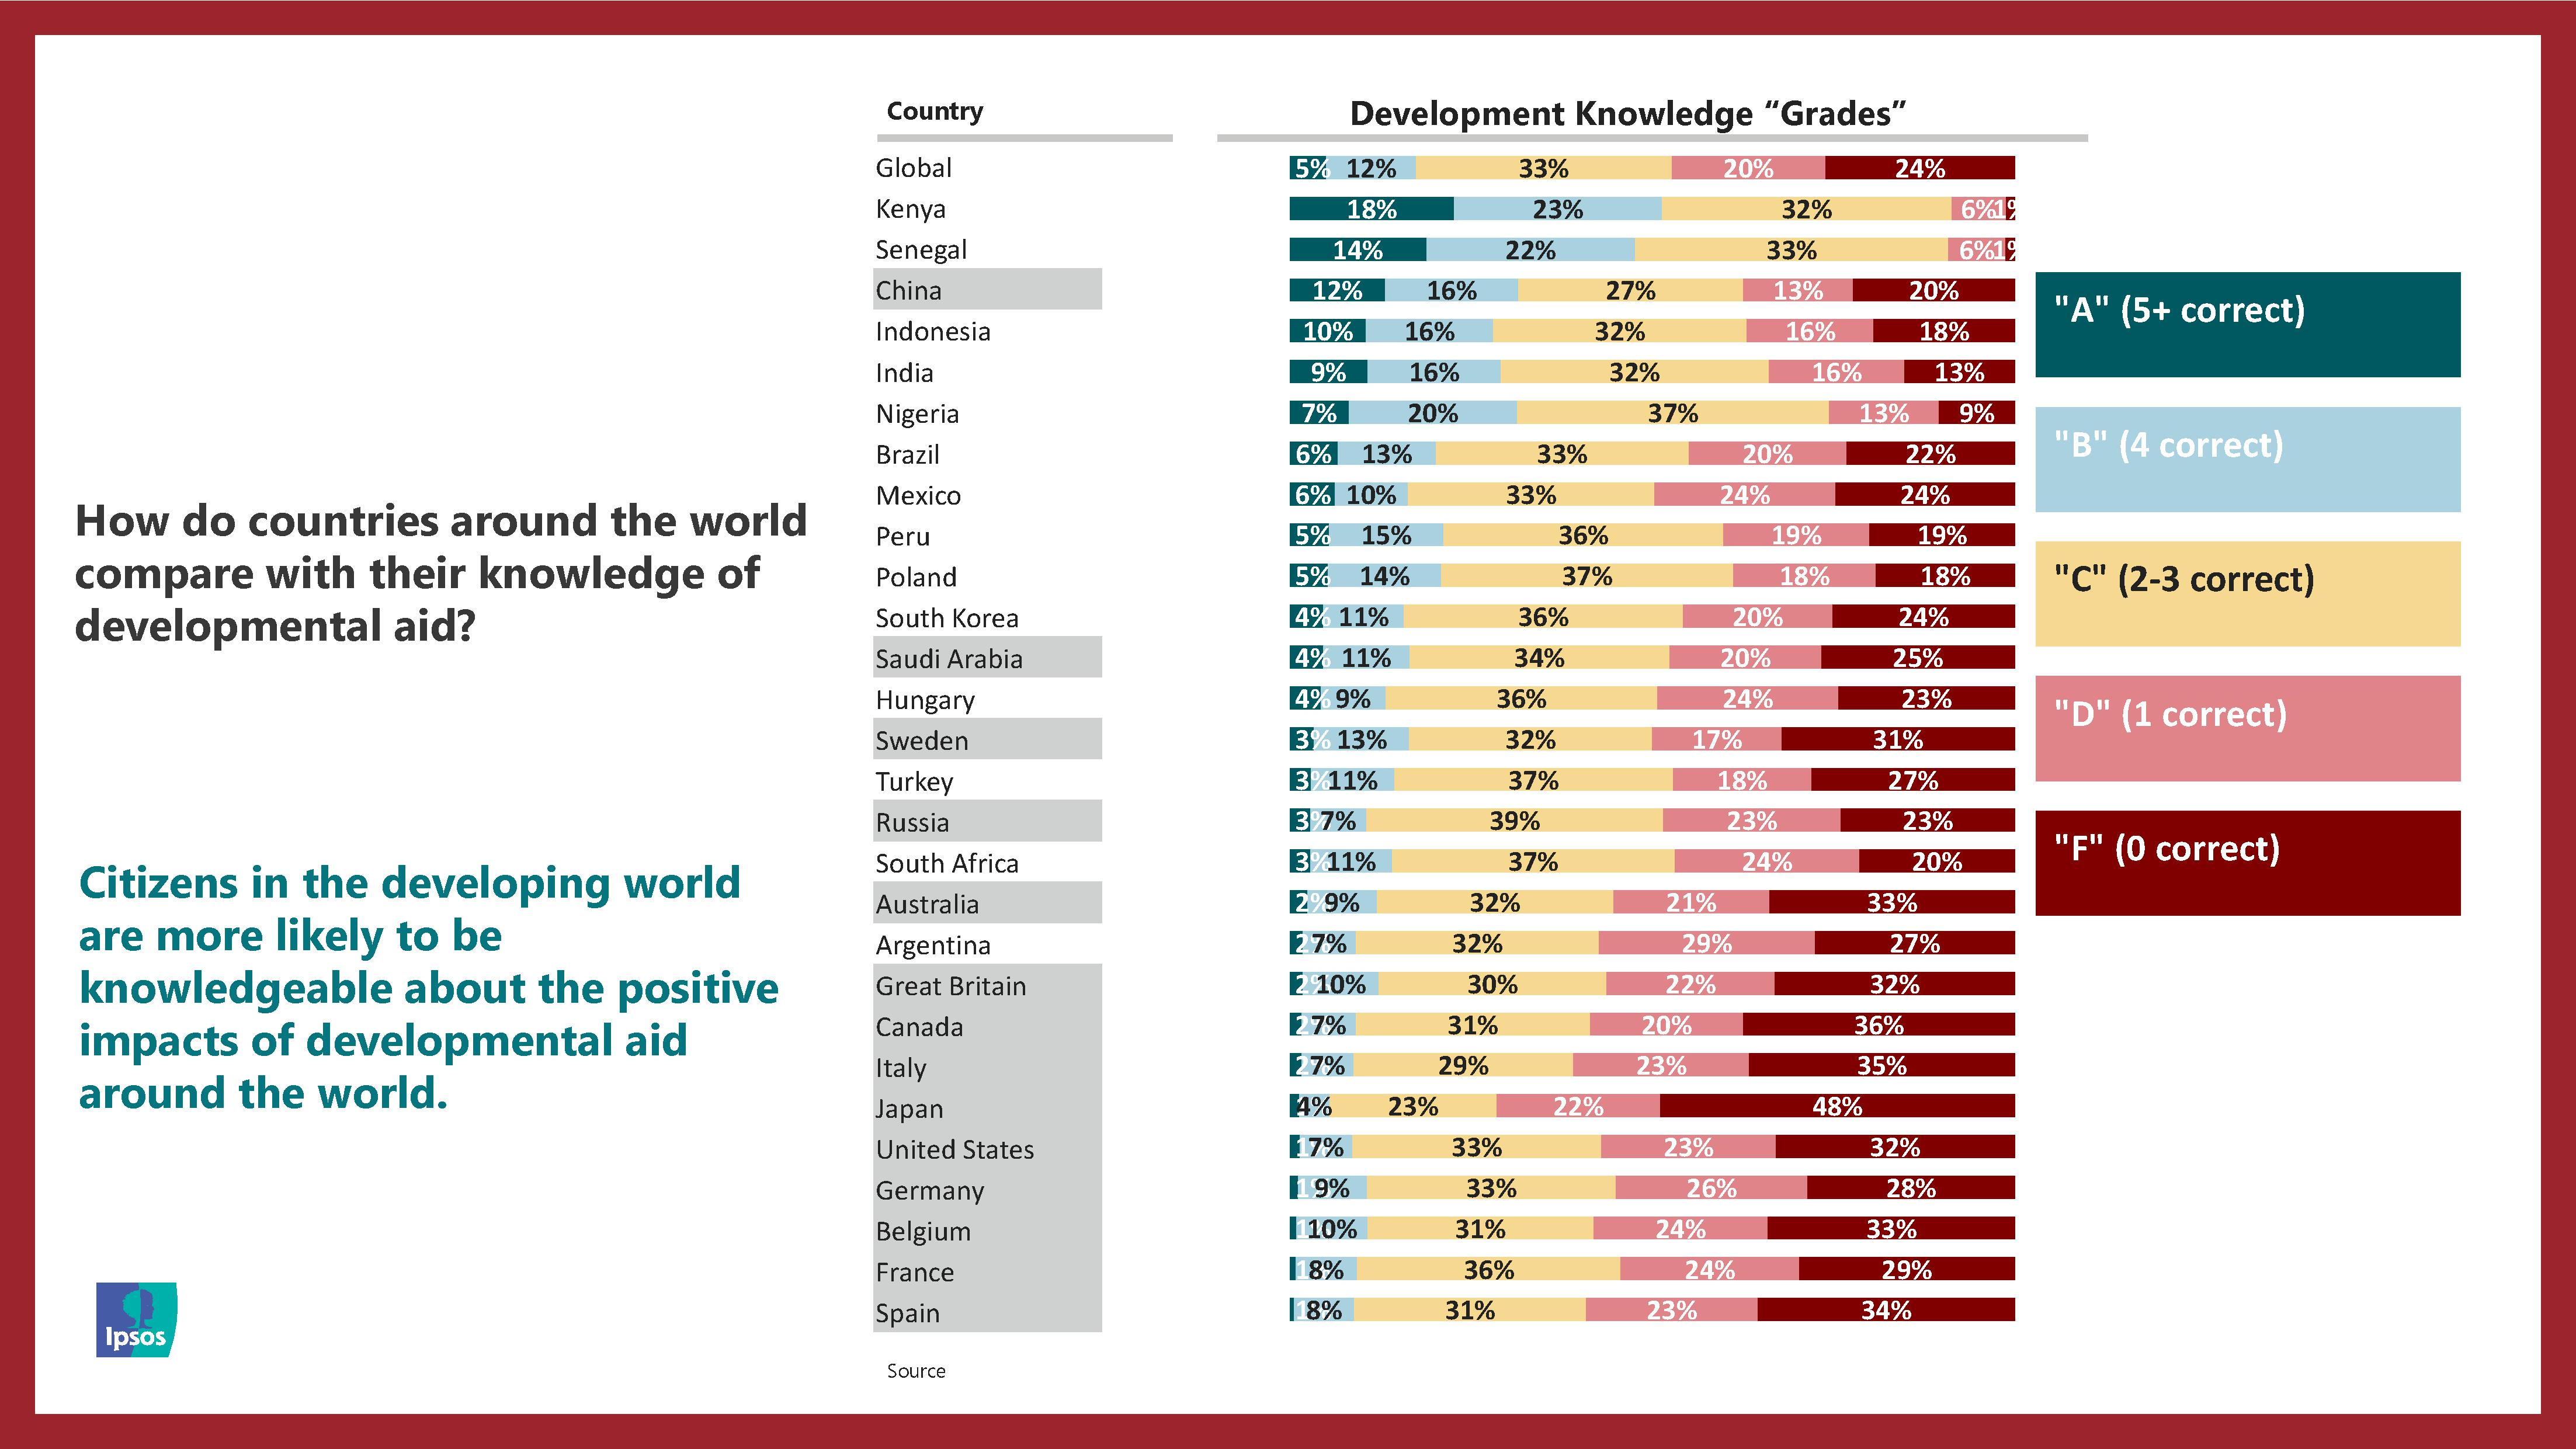
\includegraphics[width=\textwidth]{03MarcoTeorico/imageR/ipso}
	\caption{Gráfica global de la percepción de 28 paises respecto a la realidad. Donde vemos una gráfica que representa la cantidad de aciertos que tuvo la población por país en relación a la realidad.[Imagen](2017, Septiembre). Recuperado de https://www.ipsos.com/sites/default/files/ct/news/documents/2017-09/Gates\_Perils\_of\_Perception\_Report-September\_2017.pdf}
	\label{fig:ipso}
\end{figure}

\section{Consecuencias}
Ya que el desarrollo social y cultural están ligados, estos se encuentran también dependientes el uno del otro para su impulso. El movimiento cultural no solo favorecer el desarrollo recreativo si no que impulsa el desarrollo de sus naciones y viceversa. Tenemos como ejemplo en otros países del mundo, donde han sabido valorar las costumbres y tradiciones, he ahí donde nace el orgullo por su patria y se convierten en nacionalistas, demostrando el amor por su pueblo, marcando de manera definitiva el desarrollo científico, político y social de su nación\cite{pp06}.
\\[1pt]

La ignorancia cultural es el principal elemento que permite la injusticia, la enajenación y la explotación. Este fenómeno es sumamente grave y perjudicial para conformar lo que es la Identidad Cultural, la Identidad Nacional y la conciencia de la Nación. Al no saber quién es, cuáles son sus orígenes, su historia, su legado, su nombre, sus valores y principios, se le condena a la sociedad a permanentemente estar exaltando lo ajeno y despreciando lo propio.
\\[1pt]

En 2017, 41\% de los mexicanos no fue a ninguna actividad cultural según INEGI\cite{pp02}. La cifra podría leerse al revés: donde el 59\% del total de la población de 18 y más años de edad declaró que asistió a algún evento cultural seleccionado en los últimos doce meses. Pero cuando se trata de un país con una intensa vida cultural y artística, con más de 1,300 museos, alrededor de 178 zonas arqueológicas abiertas al público, 641 teatros y más de 4,000 salas de cine, de acuerdo con datos de la propia Secretaria de Cultura del gobierno federal\cite{pp01} al final queda que cuatro de cada diez personas no tienen como hábito la cultura a pesar de que varios de ellos son gratuitos.
\\[1pt]

Como ejemplo de la decadente autoconciencia cultural en México tenemos el día de la independencia. Quizá podría pensarse que todos los mexicanos saben que se festeja el 15 y 16 de septiembre. Sin embargo, los datos de la encuesta telefónica de Parametría\cite{pp03} muestran que 11\% de las personas no tiene idea de lo que se conmemora como se ve en la gráfica \ref{fig:enc01} y 57\% no sabe de que país se independizó como se ve en la gráfica \ref{fig:enc02}. Adicionalmente como podría esperarse, el nivel de escolaridad influye en el conocimiento que se tiene sobre el tema. Así, puede observarse que conforme aumenta el nivel de escolaridad se incrementa el conocimiento sobre la celebración de independencia y también sobre el país del cual se independizó México según la gráfica. \ref{fig:enc03}.
\\[1pt]

\begin{figure}
	\centering 
	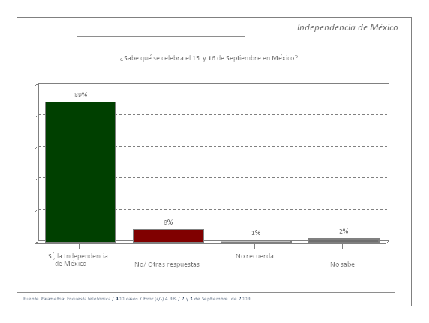
\includegraphics[width=.50\textwidth]{03MarcoTeorico/imageR/enc01}
	\caption{Gráfica a la pregunta ¿Sabe que se celebra el 15 y 16 de Septiembre en México?[Imagen](2009, Septiembre). Recuperado de: http://www.parametria.com.mx/carta\_parametrica.php?cp=4170.}
	\label{fig:enc01}
\end{figure}

\begin{figure}
	\centering 
	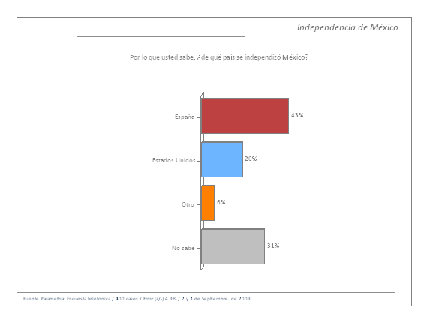
\includegraphics[width=.5\textwidth]{03MarcoTeorico/imageR/enc02}
	\caption{Gráfica a la pregunta ¿De que país se independizó México?[Imagen](2009, Septiembre). Recuperado de: http://www.parametria.com.mx/carta\_parametrica.php?cp=4170.}
	\label{fig:enc02}
\end{figure}

\begin{figure}
	\centering 
	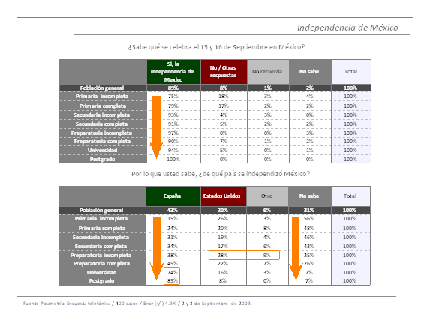
\includegraphics[width=.5\textwidth]{03MarcoTeorico/imageR/enc03}
	\caption{Gráfica de como influye la escolaridad en el conocimiento que se tiene de las fiestas patrias[Imagen](2009, Septiembre). Recuperado de: http://www.parametria.com.mx/carta\_parametrica.php?cp=4170.}
	\label{fig:enc03}
\end{figure}

Debemos saber cuál es nuestra verdadera herencia cultural y cuál nuestro legado, para preservarlo y desarrollarlo. Y como dice Guillermo Marín \cite{pp07} ``Este país se tiene que encontrar a sí mismo".
\\[1pt]


\section{Propuesta de solución}
Propondremos como solución el crear un videojuego con contexto histórico y mitológico del país prehispánico mexicano. Para esto el factor de entretenimiento y diversión lo sobrepondremos al del conocimiento o educativo.
\\[1pt]

%%%%%%%%%%%%%%%%%%%%%%%%%5YA EXISTE?
Como ejemplo similar tomaremos el videojuego llamado ``Assasins Creed II" lanzado en el año 2009, que debutó en el puesto número 1 en Estados Unidos, Canadá, Suecia, Francia, España y Australia, y dentro del «Top 50» en más de diez países. Este juego tiene como género acción-aventura, también se situa en la época renacentista y este hecho lográ que el jugador adquiera conocimientos sobre ese tiempo, tanto lugares, como personas, situación social, etc.
\\[1pt]

%%%%%%%%%%%%%%%%%%%%%%%%%%55QUE IMPLICA?
Para llevar a cabo el diseño de un videojuego los programadores son los responsables de hacer posible la interactividad entre el jugador y el sistema. Se realizará detro del proyecto la programación estructurada, orientada a objetos, modelado, arte digital, conocimiento de dispositivos móviles y animación digital. Considerando importante usar modelos matemáticos para las diferentes experiencias de juego. 
\\[1pt]

%%%%%%%%%%%%%%%%%%%%%%%%%%%%%%%VENTAJAS?
El resultado de adquisición de conocimiento en lo videojuegos se debe al cómo. En la imagen \ref{fig:conoAprendizaje} se muestra el cono de la experiencia de Edgar Dale (pedagogo) donde resaltamos que el mayor aprendizaje es por medio de la simulación.

\begin{figure}
	\centering 
	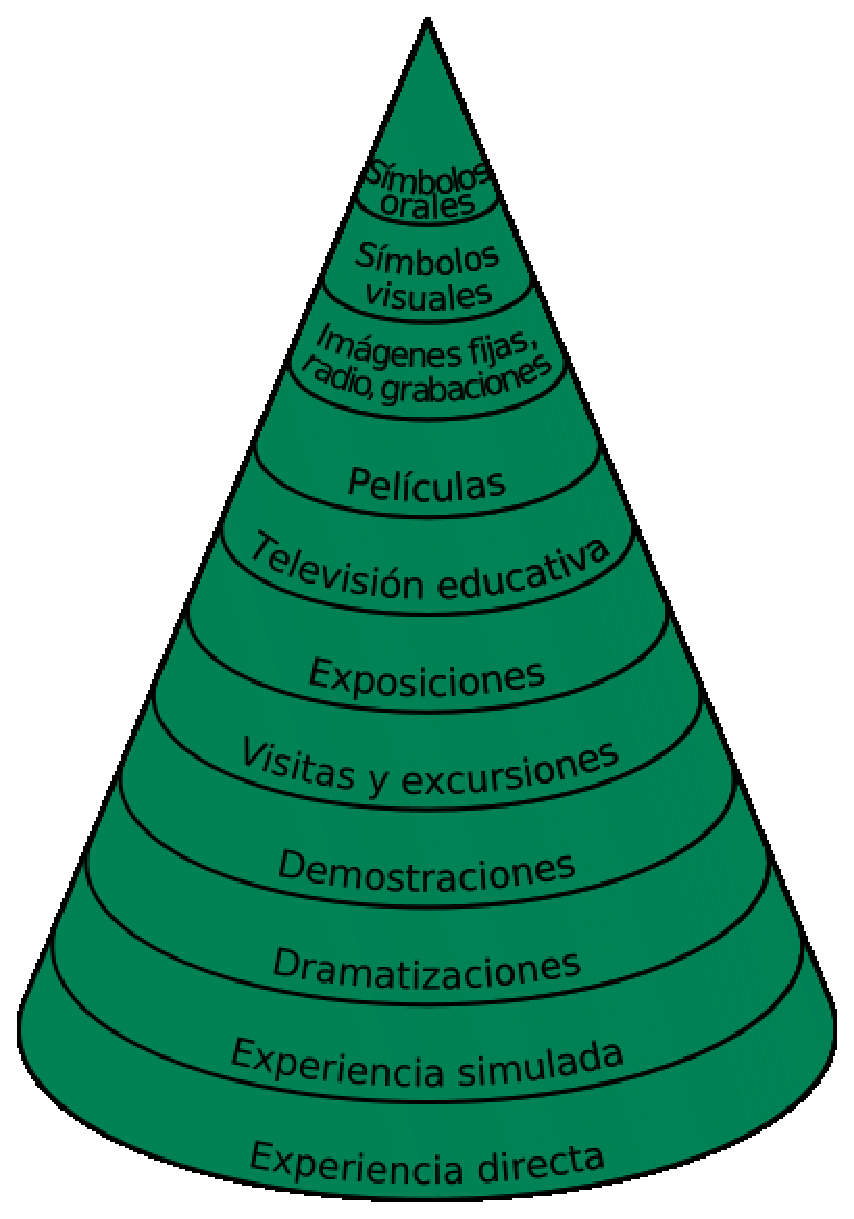
\includegraphics[width=.5\textwidth]{03MarcoTeorico/imageR/conoAprendizaje}
	\caption{Cono de la experiencia de Edgar Dale. Se muestra diferentes maneras de aprendizaje que se ordenan según su impacto de aprendizaje.[Imagen](2008). Recuperado de: https://es.wikipedia.org/wiki/Edgar\_Dale\#/media/File:Cono\_de\_la\_Experiencia.svg}
	\label{fig:conoAprendizaje}
\end{figure}

Los medios audiovisuales son los que mayor impacto tiene en difusión cultural como se ve en la gráfica de la imagen \ref{fig:modecult}. Así podemos ver una potencial herramienta para insitar a la participación en los eventos culturales, pues los videojuegos son medios audiovisuales.
\\[1pt]

\begin{figure}
	\centering 
	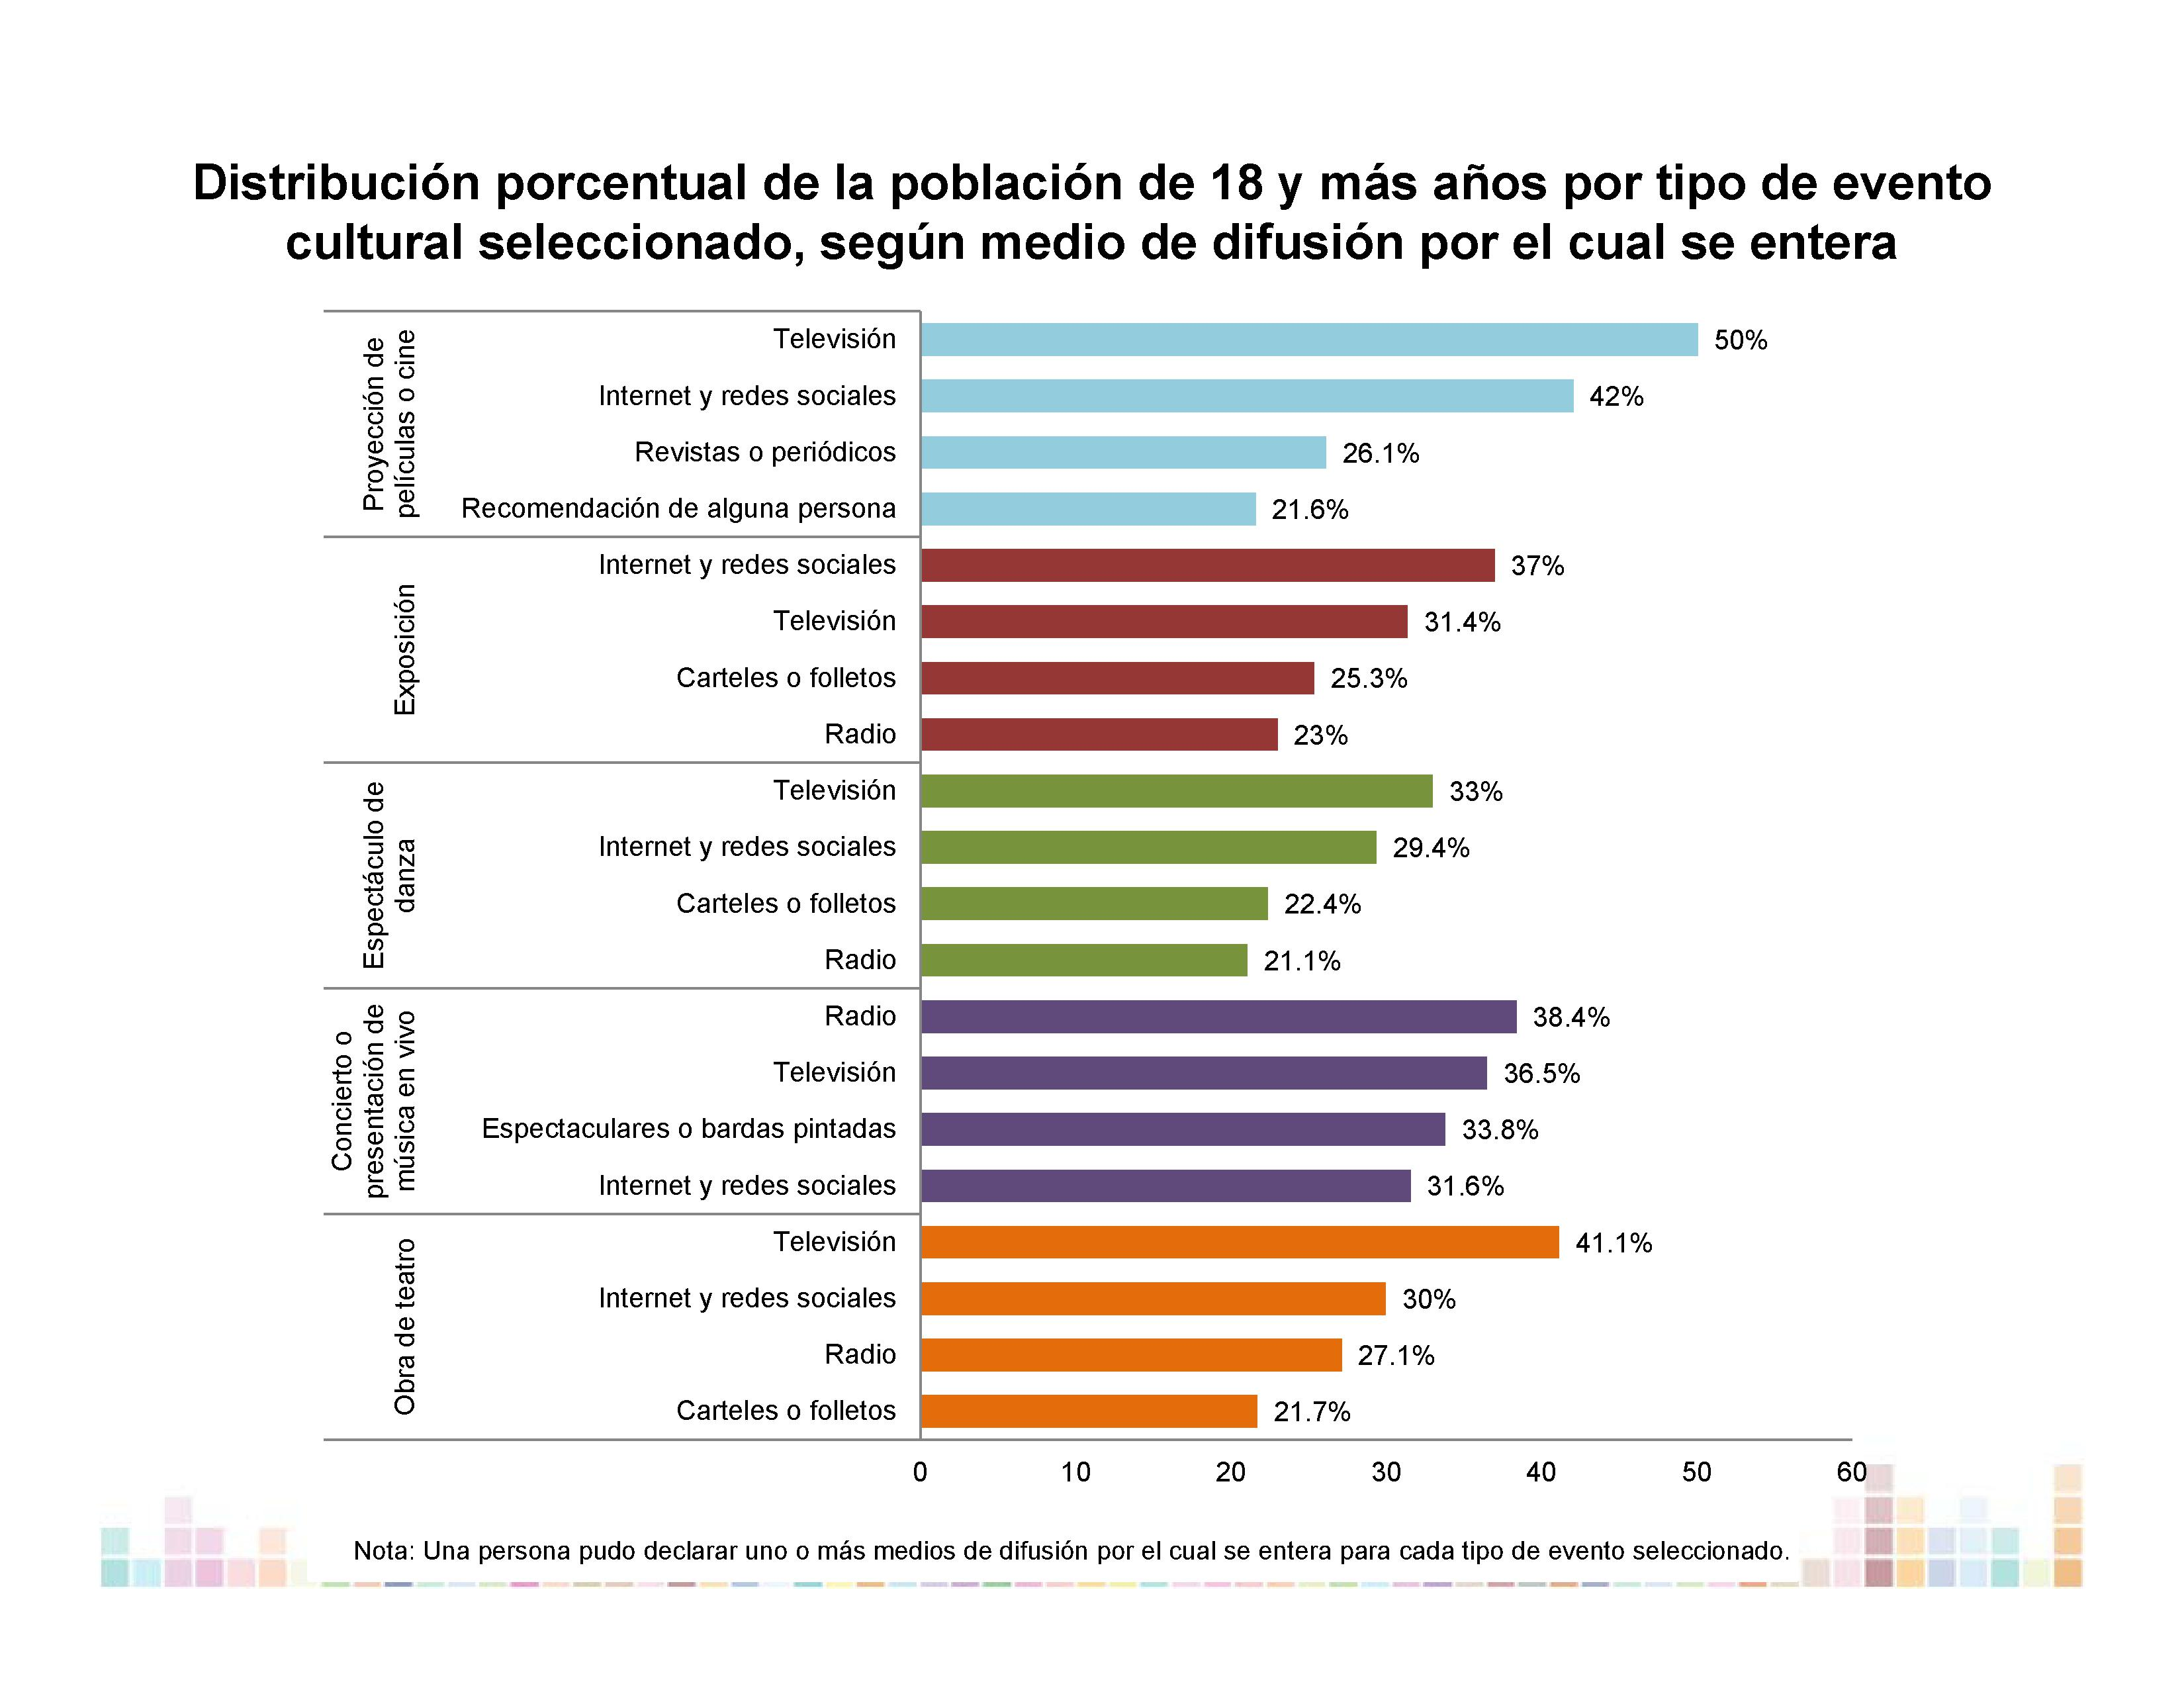
\includegraphics[width=.75\textwidth]{03MarcoTeorico/imageR/modecult}
	\caption{Encuesta MODECULT en asistencia por tipo de evento y medio de difusión por el cual se ha enterado.[Imegen](2017, Mayo). Recuperado de: http://internet.contenidos.inegi.org.mx/contenidos/productos/prod\_serv/contenidos/espanol/bvinegi/productos/nueva\_estruc/promo/resultados\_modecult\_may2017.pdf}
	\label{fig:modecult}
\end{figure}

También otra de las ventajas es la cantidad de gente que juega videojuegos en México y el dispositivo por el cuál lo consumen como lo muestra la imagen \ref{fig:consumo30}. Donde el 20\% de los mexianos consumen videojuegos y 45\% de ellos se juegan en dispositivos móviles.

\begin{figure}
	\centering 
	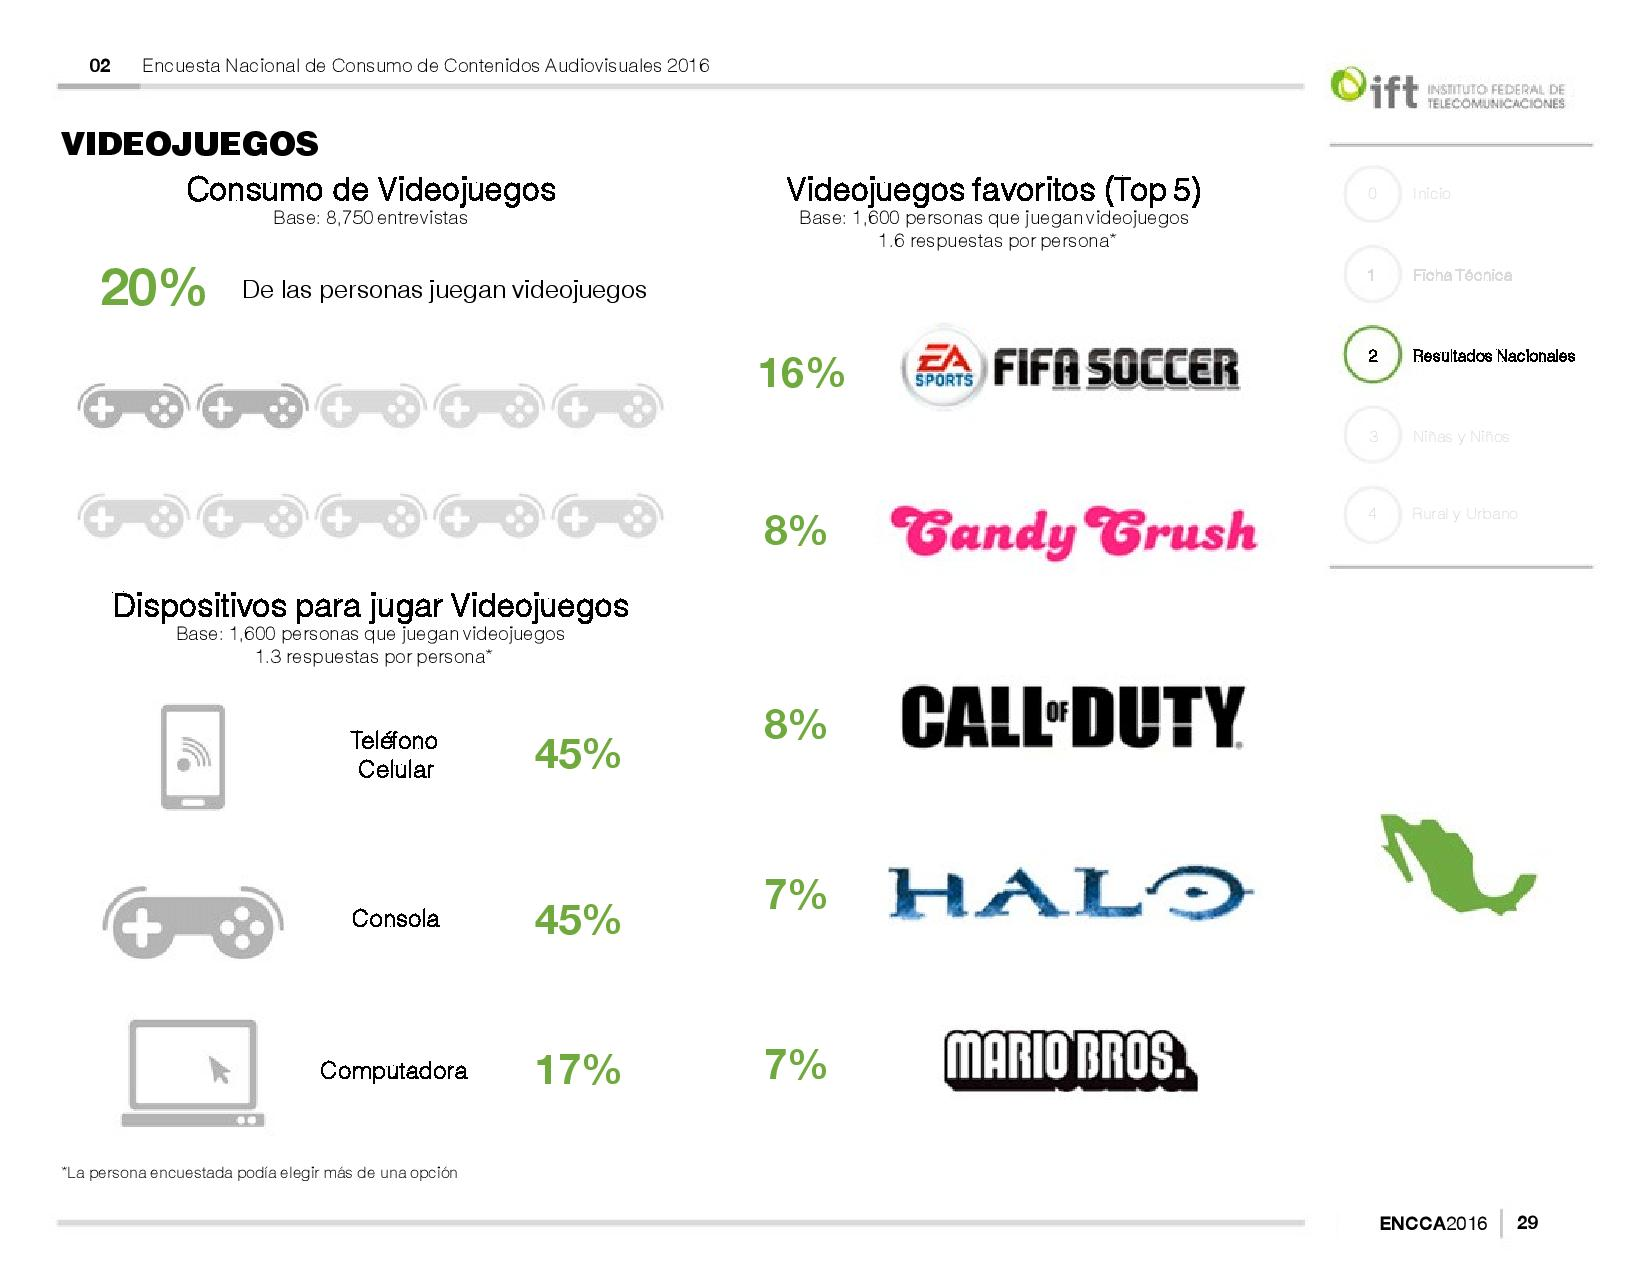
\includegraphics[width=.75\textwidth]{03MarcoTeorico/imageR/consumo30}
	\caption{Encuesta Nacional de Consumo de Contenidos Audiovisuales, donde muestra el consumo de videojuegos[Imegen](2016). Recuperado de: http://www.ift.org.mx/sites/default/files/encca2016\_vf-compressed.pdf}
	\label{fig:consumo30}
\end{figure}

%%%%%%%%%%%%%%%%%%%%%%%%%%DESVENTAJAS?

Una desventaja de los videojuegos en cuestión de desarrollo es que son un complejo sistema tecnológico que combina diversos elementos: visuales, matemáticos, físicos, electrónicos o narrativos, entre otros muchos para generar una experiencia controlada porel jugador para su mayor entretenimiento. Por tanto existe una complejidad al unir de forma adecuada todos esos elemntos para crear una gran experiencia de diversión para los jugadores, se necesita de una gran cantidad de talentos diversos o multidisciplinarios, los cuales no se abarcarán todos ellos.

También se debe tomar en cuenta que existe una gran cantidad de gustos e intereses entre los jugadores existentes y no se puede aplicar todos los existentes.

La mejora de las condiciones de un producto en un videojuego resulta esencial. Por esta misma razón el tiempo de desarrollo siempre es muy largo y en la mayoría de las ocasiones tiene muchos contratiempos que provocan retrasos de lanzamiento o incluso rediseños completos.



